\documentclass{article}
\usepackage{tikz}
\usetikzlibrary{positioning}
\usetikzlibrary{decorations.markings}
\usepackage[dvipsnames]{xcolor}
\usepackage{amsmath}

\begin{document}

\title{Matrizen in Neuronalen Netzwerken}
\author{Tim Zollner}
\date{17.02.2025}
\maketitle

\section{Grafik}
    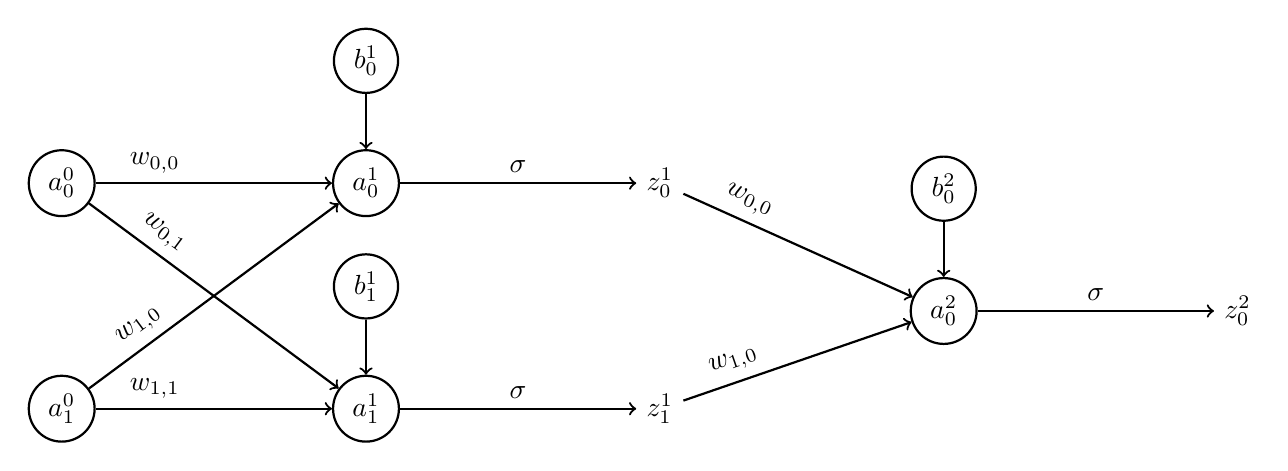
\begin{tikzpicture} [thick, main/.style = {draw, circle}]
        %Knoten
        \node[main] (00) {$a_0^0$};
        \node[main] (01) [below = 2cm of 00] {$a_1^0$};

        \node[main] (10) [right = 3cm of 00] {$a_0^1$};
        \node[main] (11) [right = 3cm of 01] {$a_1^1$};

        \node[main] (b10) [above = 0.7cm of 10] {$b_0^1$};
        \node[main] (b11) [above = 0.7cm of 11] {$b_1^1$};

        \node (z10) [right = 3cm of 10] {$z_0^1$};
        \node (z11) [right = 3cm of 11] {$z_1^1$};

        \node[main] (20) [below right = 1cm and 3cm of z10] {$a_0^2$};
        \node[main] (b20) [above = 0.7cm of 20] {$b_0^2$};

        \node (z20) [right = 3cm of 20] {$z_0^2$};

        %Kanten
        \draw[->] (00) -- (10) node[pos=0.25, above] {$w_{0,0}$};
        \draw[->] (00) -- (11) node[pos=0.25, above, sloped] {$w_{0,1}$};
        \draw[->] (01) -- (10) node[pos=0.25, above, sloped] {$w_{1,0}$};
        \draw[->] (01) -- (11) node[pos=0.25, above] {$w_{1,1}$};

        \draw[->] (b10) -- (10);
        \draw[->] (b11) -- (11);

        \draw[->] (10) -- (z10) node[midway, above] {$\sigma$};
        \draw[->] (11) -- (z11) node[midway, above] {$\sigma$};


        \draw[->] (z10) -- (20) node[pos=0.25, above, sloped] {$w_{0,0}$};
        \draw[->] (z11) -- (20) node[pos=0.25, above, sloped] {$w_{1,0}$};

        \draw[->] (b20) --(20);

        \draw[->] (20) -- (z20) node[midway, above] {$\sigma$};



    \end{tikzpicture}

\section{Formeln}

\[ a_0^1 = a_0^0 \cdot \textcolor{OliveGreen}{w_{0,0}} + a_1^0 \cdot \textcolor{OliveGreen}{w_{1,0}} + \textcolor{blue}{b^1} \]
allgemein:
\[  a_0^1 = \textcolor{blue}{b^1} + \sum_{k=0}^{n} a_k^0 \cdot \textcolor{OliveGreen}{w_{k,0}}  \]

\[z_n^m = \sigma(a_n^m)\]

\[\sigma(x) = \frac{1}{1 + e^{-t}}\]

\[W_{max} = [-1;1]\]


\section{Matrizendarstellung}

\[ \vec{a}_m = \left(\begin{array}{c} a_0^m \\ a_1^m \\ ... \\ a_n^m \end{array}\right) 
\kern 50pt
\vec{b}_m = \left(\begin{array}{c} b_0^m \\ b_1^m \\ ... \\ b_n^m \end{array}\right) 
\kern 50pt
W = \begin{pmatrix}
    w_{0,0} & w_{1,0} & ... & w_{n,0} \\
    w_{0,1} & w_{1,1} & ... & w_{n,1} \\
    ... & ... & ... & ... \\
    w_{0,j} & w_{1,j} & ... & w_{n,j}
\end{pmatrix} \]

\[ \vec{a}_m = \vec{a}_{m-1} \cdot W + \vec{b}_m \]

\[ 
\left(\begin{array}{c} a_0^m \\ a_1^m \\ ... \\ a_n^m \end{array}\right)
=
\left(\begin{array}{c} a_0^{m-1} \\ a_1^{m-1} \\ ... \\ a_n^{m-1} \end{array}\right)
\cdot
\begin{pmatrix}
    w_{0,0} & w_{1,0} & ... & w_{n,0} \\
    w_{0,1} & w_{1,1} & ... & w_{n,1} \\
    ... & ... & ... & ... \\
    w_{0,j} & w_{1,j} & ... & w_{n,j}
\end{pmatrix}
+
\left(\begin{array}{c} b_0^m \\ b_1^m \\ ... \\ b_n^m \end{array}\right)
 \]

 \[
\left(\begin{array}{c} a_0^m \\ a_1^m \\ ... \\ a_n^m \end{array}\right)
=
\left(\begin{array}{c}
    w_{0,0} \cdot a_0^{m-1} + w_{1,0} \cdot a_1^{m-1} + ... + w_{n,0} \cdot a_n^{m-1} \\
    w_{0,1} \cdot a_0^{m-1} + w_{1,1} \cdot a_1^{m-1} + ... + w_{n,1} \cdot a_n^{m-1} \\
    ... \\
    w_{0,j} \cdot a_0^{m-1} + w_{1,j} \cdot a_1^{m-1} + ... + w_{n,j} \cdot a_n^{m-1}
\end{array}\right)
+
\left(\begin{array}{c} b_0^m \\ b_1^m \\ ... \\ b_n^m \end{array}\right)
\]
\[ a = b \kern 50pt c = d \]



\end{document}